\documentclass[12pt,letterpaper]{article}
\usepackage[utf8]{inputenc}
\usepackage[spanish, es-tabla]{babel}
\usepackage[version=3]{mhchem}
\usepackage[journal=jacs]{chemstyle}
\usepackage{graphicx}
\usepackage{amsmath}
\usepackage{amsfonts}
\usepackage{amssymb}
\usepackage{makeidx}
\usepackage{xcolor}
\usepackage[stable]{footmisc}
\usepackage[section]{placeins}
%Paquetes necesarios para tablas
\usepackage{longtable}
\usepackage{array}
\usepackage{xtab}
\usepackage{multirow}
\usepackage{colortab}
%Paquete para el manejo de las unidades
\usepackage{siunitx}
\sisetup{mode=text, output-decimal-marker = {,}, per-mode = symbol, qualifier-mode = phrase, qualifier-phrase = { de }, list-units = brackets, range-units = brackets, range-phrase = --}
\DeclareSIUnit[number-unit-product = \;] \atmosphere{atm}
\DeclareSIUnit[number-unit-product = \;] \pound{lb}
\DeclareSIUnit[number-unit-product = \;] \inch{"}
\DeclareSIUnit[number-unit-product = \;] \foot{ft}
\DeclareSIUnit[number-unit-product = \;] \yard{yd}
\DeclareSIUnit[number-unit-product = \;] \mile{mi}
\DeclareSIUnit[number-unit-product = \;] \pint{pt}
\DeclareSIUnit[number-unit-product = \;] \quart{qt}
\DeclareSIUnit[number-unit-product = \;] \flounce{fl-oz}
\DeclareSIUnit[number-unit-product = \;] \ounce{oz}
\DeclareSIUnit[number-unit-product = \;] \degreeFahrenheit{\SIUnitSymbolDegree F}
\DeclareSIUnit[number-unit-product = \;] \degreeRankine{\SIUnitSymbolDegree R}
\DeclareSIUnit[number-unit-product = \;] \usgallon{galón}
\DeclareSIUnit[number-unit-product = \;] \uma{uma}
\DeclareSIUnit[number-unit-product = \;] \ppm{ppm}
\DeclareSIUnit[number-unit-product = \;] \eqg{eq-g}
\DeclareSIUnit[number-unit-product = \;] \normal{\eqg\per\liter\of{solución}}
\DeclareSIUnit[number-unit-product = \;] \molal{\mole\per\kilo\gram\of{solvente}}
\usepackage{cancel}
%Paquetes necesarios para imágenes, pies de página, etc.
\usepackage{graphicx}
\usepackage{lmodern}
\usepackage{fancyhdr}
\usepackage[left=4cm,right=2cm,top=3cm,bottom=3cm]{geometry}

%Instrucción para evitar la indentación
%\setlength\parindent{0pt}
%Paquete para incluir la bibliografía
\usepackage[backend=bibtex,style=chem-acs,biblabel=dot]{biblatex}
\addbibresource{references.bib}

%Formato del título de las secciones

\usepackage{titlesec}
\usepackage{enumitem}
\titleformat*{\section}{\bfseries\large}
\titleformat*{\subsection}{\bfseries\normalsize}

%Creación del ambiente anexos
\usepackage{float}
\floatstyle{plaintop}
\newfloat{anexo}{thp}{anx}
\floatname{anexo}{Anexo}
\restylefloat{anexo}
\restylefloat{figure}

%Modificación del formato de los captions
\usepackage[margin=10pt,labelfont=bf]{caption}

%Paquete para incluir comentarios
\usepackage{todonotes}

%Paquete para incluir hipervínculos
\usepackage[colorlinks=true, 
            linkcolor = blue,
            urlcolor  = blue,
            citecolor = black,
            anchorcolor = blue]{hyperref}

\setcounter{equation}{0} %RESET DEL CONTADOR DE ECUACIONES 
 
%%%%%%%%%%%%%%%%%%%%%%%%%%%%%%%%%%%%%%%%%%%%%%%%%%%%%%%%%%%%%%%%%%%%%
%Inicio del documento%
%%%%%%%%%%%%%%%%%%%%%%%%%%%%%%%%%%%%%%%%%%%%%%%%%%%%%%%%%%%%%%%%%%%%%


\begin{document}

\renewcommand{\labelitemi}{$\checkmark$}
\renewcommand{\CancelColor}{\color{red}}
\newcolumntype{L}[1]{>{\raggedright\let\newline\\\arraybackslash}m{#1}}
\newcolumntype{C}[1]{>{\centering\let\newline\\\arraybackslash}m{#1}}
\newcolumntype{R}[1]{>{\raggedleft\let\newline\\\arraybackslash}m{#1}}


\begin{figure}[h!]
\begin{floatrow}
%\caption{Poderosisima udeg}
\centering

\includegraphics[width=2.6cm]{udg.png}
\label{fig:tubes}
\end{floatrow}
\end{figure}




\begin{center}
	\textbf{\LARGE{Universidad de Guadalajara}}\\
	\vspace{2mm}
		\textbf{\large{Jose Luis Tlaloc Sauceda Alvarez}}\\
	\vspace{2mm}
	\textbf{\large{Ingeniería de control}}
		\vspace{2mm}
	
	\today
\end{center}
\vspace{4mm}

%%%%%%%%%%%%%%%%%%%%%%%%%%%%%%%%%%%%%%%%%%%%%%%%%%%%%%%%%%%%%%%%%%%%%%%%%%%%%%%%%%%%%%%%%%%%%%%%%%%%%%%%%%%%%%%%%%%%%%%%%
\section*{\centering Control PID} %TITULO
%%%%%%%%%%%%%%%%%%%%%%%%%%%%%%%%%%%%%%%%%%%%%%%%%%%%%%%%%%%%%%%%%%%%%%%%%%%%%%%%%%%%%%%%%%%%%%%%%%%%%%%%%%%%%%%%%%%%%%%%%


\section{Resumen}

La siguiente actividad busca que el estudiante disẽne un controlador PID. Adeḿas, utilizar el software de MATLAB para comprobación de los calculos. 
%%%%%%%%%%%%%%%%%%%%%%%%%%%%%%%%%%%%%%%%%%%%%%%%%%%%%%%%%%%%%%%%%%%%%%%%%%%%%%%%%%%%%%%%%%%%%%%%%%%%%%%%%%%%%%%%%%%%%%%%%

\section{Introducción}

Un controlador PID es un mecanismo de control simultáneo por realimentación ampliamente. Este calcula la desviación o error entre un valor medido y un valor deseado. 

El algoritmo del control PID consta de tres parámetros distintos: el proporcional, el integral, y el derivativo. El valor proporcional depende del error actual, el integral depende de los errores pasados y el derivativo es una predicción de los errores futuros. La suma de estas tres acciones es usada para ajustar el proceso por medio de un elemento de control como un actuador.


\begin{figure}[h]
  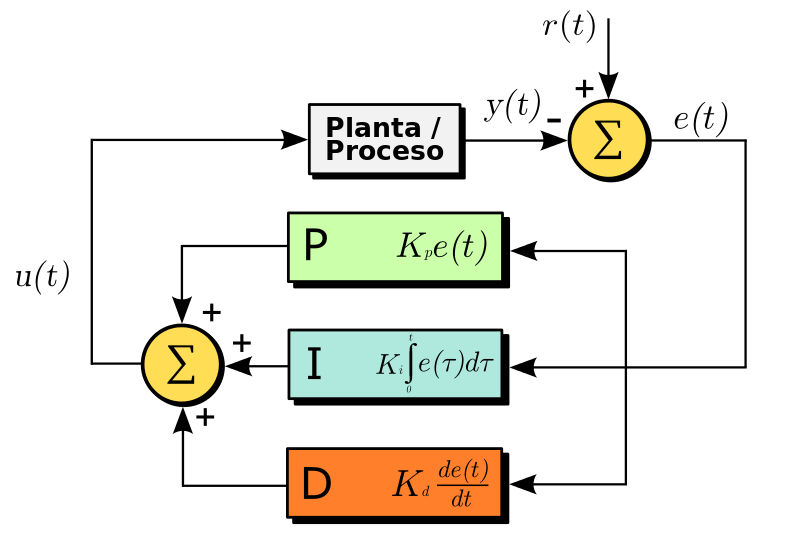
\includegraphics[scale= 0.23]{pid.png}
  %\caption{Diagrama de bloques simplificado}
  \label{fig:Bloques}
\end{figure} \\  

\textbf{Actividad: Diseñar un controlador PID para cada una de las siguientes funciones de transferencia tomando en consideración los parametros de diseño \%OS y T_{s}. \ Asumiendo \ n = 9; }


\begin{equation}\frac{n}{s+n} = \frac{9}{s+9} \quad \mathrm{OS}=10 \%, \mathrm{Ts}=3 \mathrm{s}\end{equation} 

\begin{equation}\frac{2n}{4s+n} = \frac{4.5}{s+2.25} \quad \mathrm{OS}=1 \%, \mathrm{Ts}=1 \mathrm{s}\end{equation} 

\begin{equation}\frac{3n}{4s+5} = \frac{6.75}{s+1.25} \quad \mathrm{OS}=15 \%, \mathrm{Ts}=0.1 \mathrm{s}\end{equation} 

\begin{equation}\frac{4n}{2s^{2}+4s+6} = \frac{18}{s^{2}+2s+3} \quad \mathrm{OS}=20 \%, \mathrm{Ts}=10 \mathrm{s}\end{equation} \\ 


%%%%%%%%%%%%%%%%%%%%%%%%%%%%%%%%%%%%%%%%%%%%%%%%%%%%%%%%%%%%%%%%%%%%%%%%%%%%%%%%%%%%%%%%%%%%%%%%%%%%%%%%%%%%%%%%%%%%%%%%%%
\section{Metodología}
\setcounter{equation}{0} %RESET DEL CONTADOR DE ECUACIONES 

Los siguientes pasos permitiran diseñar rapidamente controladores PID mediante la técnica de asignación de polos. \\ 

\textbf{Paso 1: Calcular G(s)_{ideal} }: \\ 

Para esto utilizamos el modelo de una función de transferencia de segundo orden. La idea es aproximar una función de transferencia ideal que cumpla con los parametros de diseño establecidos.  \\ 

* Paso 1.1 calcular \zeta.

\begin{equation}\zeta=\frac{- \ln(\%OS / 100)}{\sqrt{\pi^{2}+\ln(\%OS / 100)^{2}}}\end{equation} 

* Paso 1.2 calcular \omega_{n}. 

\begin{equation}\omega_{n}=\frac{4}{\zeta \ T_{s}}\end{equation}  \\

* Paso 1.3 sustituir zeta y omega en G(s)_{ideal}. \\ 

\begin{equation}G(s)_{ideal}=\frac{V_{f} \omega_{n}^{2}}{s^{2}+2 \omega_{n}\zeta s+w_{n}^{2}}\end{equation} \\ 

\setcounter{equation}{0} %RESET DEL CONTADOR DE ECUACIONES 
\textbf{Paso 2: Reducir el sistema para obtener G(s)_{general} }: \\

Donde el controlador PID esta descrito por la expresión:  \\ 

\begin{equation}H(s)=\frac{Ds^{2}+Ps+I}{s}\end{equation} \\

\begin{figure}[h]
  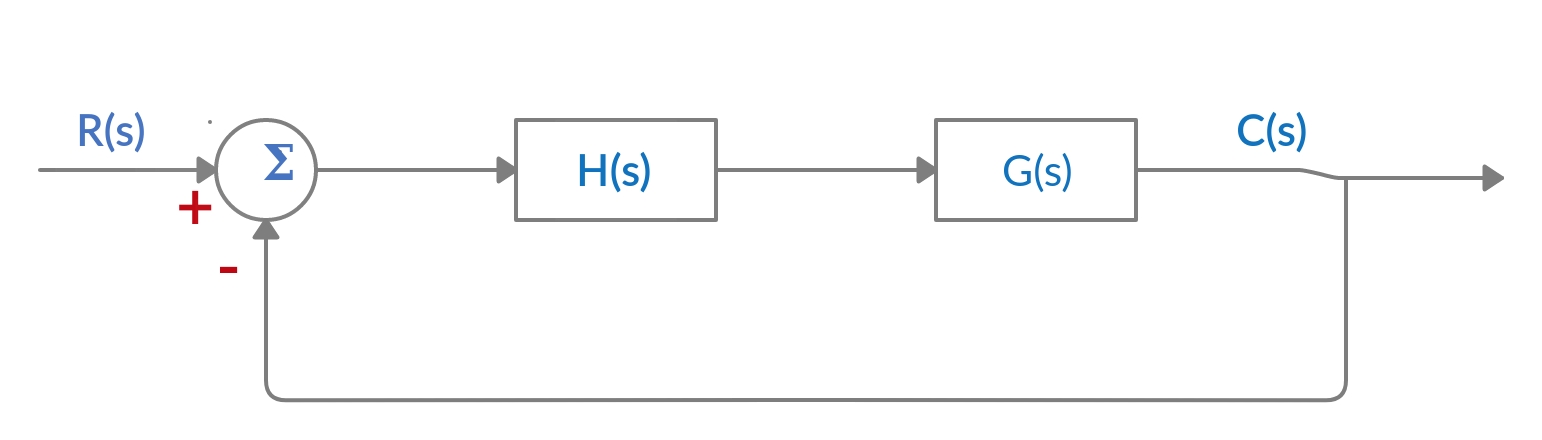
\includegraphics[scale= 0.19]{tfpid.png}
  %\caption{Diagrama de bloques simplificado}
  \label{fig:Bloques}
\end{figure} \\  


Se busca simplificar el sistema en su minima expresión  representando el sistema con un solo bloque que describa su comportamiento con un posible controlador PID representado de forma general. \\ 

* Paso 2.1 Multiplicar bloques H(s) y G(s). \\

\begin{figure}[h]
  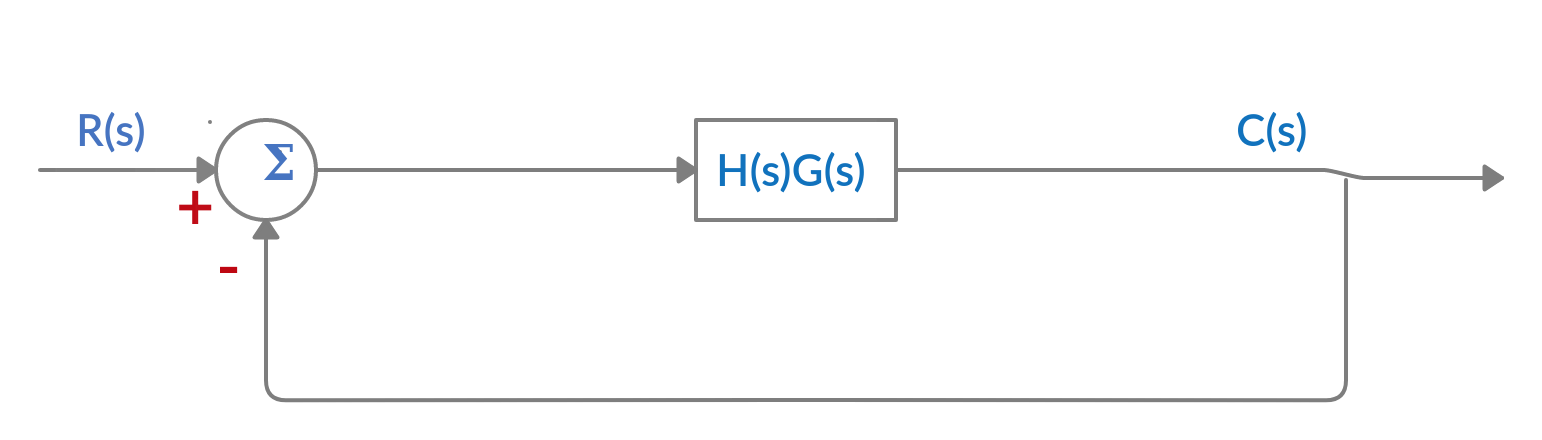
\includegraphics[scale= 0.19]{tfpid1.png}
  %\caption{Diagrama de bloques simplificado}
  \label{fig:Bloques}
\end{figure} \\  


* Paso 2.2 Simplificar retroalimentación.

\begin{figure}[h]
  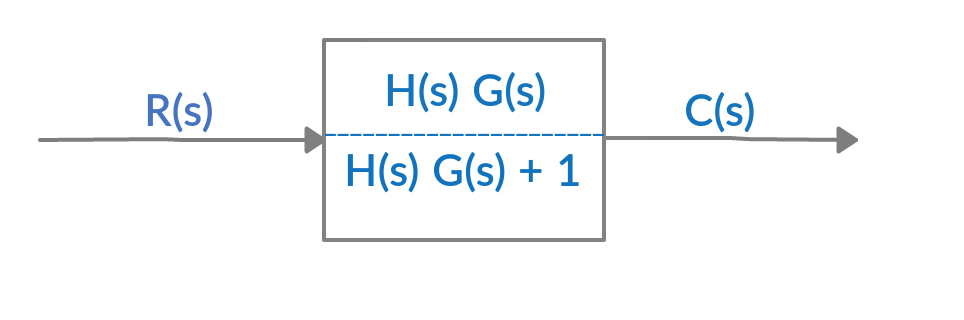
\includegraphics[scale= 0.19]{tfpid2.png}
  %\caption{Diagrama de bloques simplificado}
  \label{fig:Bloques}
\end{figure} \\  

\begin{equation}G(s)_{general} =  \frac{H(s)G(s)}{H(s)G(s) +1}\end{equation} \\ 


\setcounter{equation}{0} %RESET DEL CONTADOR DE ECUACIONES 

\textbf{Paso 3: Igualar  {G(s)_{ideal} \ y \ G(s)_{general}} } \\  

Este paso es muy importante porque al igualar ambas funciones encontraremos los valores, P, I y D para que nuestra función de transferencia ideal cumpla la igualdad con nuestra función de transferencia general. En pocas palabras, estamos asignando polos a nuestro sistema para que tenga la respuesta ideal o deseada segun nuestros parametros de diseño. \\ 

\begin{equation}G(s)_{ideal}=\frac{V_{f} \omega_{n}^{2}}{s^{2}+2 \omega_{n}\zeta s+w_{n}^{2}}\end{equation} \\ 
 
\begin{equation} G(s)_{general} =  \frac{H(s)G(s)}{H(s)G(s) +1}\end{equation} \\ 

\begin{equation}
    \frac{V_{f} \omega_{n}^{2}}{s^{2}+2 \omega_{n}\zeta s+w_{n}^{2}} =  \frac{H(s)G(s)}{H(s)G(s) +1} 
\end{equation} \\

* Paso 4 Crear un sistema de ecuaciones \\ 
\begin{equation}
    \frac{V_{f} \omega_{n}^{2}}{s^{2}+2 \omega_{n}\zeta s+w_{n}^{2}} =  \frac{(Ds^{2} + Ps + I)G(s)}{(Ds^{2} + Ps + I)G(s) \ + 1}
\end{equation} \\


\begin{equation}\left(\begin{array}{cc}
\alpha_{1} & -\beta_{1} \\
\alpha_{2} & -\beta_{2} \\
\alpha_{3} & -\beta_{3}
\end{array}\right)\left(\begin{array}{ccc}
s^{2} & s & k_{1} \\
s^{2} & s & k_{2}
\end{array}\right)=\left(\begin{array}{ccc}
\alpha_{1} s^{2}-\beta_{1} s^{2} & \alpha_{1} s-\beta_{1} s & k_{1} \alpha_{1}-k_{2} \beta_{1} \\
\alpha_{2} s^{2}-\beta_{2} s^{2} & \alpha_{2} s-\beta_{2} s & k_{1} \alpha_{2}-k_{2} \beta_{2} \\
\alpha_{3} s^{2}-\beta_{3} s^{2} & \alpha_{3} s-\beta_{3} s & k_{1} \alpha_{3}-k_{2} \beta_{3}
\end{array}\right)\end{equation} \\ \\ 

* Paso 5 Resolver el sistema para P, I y D. \\

Nota: Verificar Matriz, posible error de modelo matematico, se iguala parametro con parametro para encontrar el valor que hace proporcional la ecuación... 

%%%%%%%%%%%%%%%%%%%%%%%%%%%%%%%%%%%%%%%%%%%%%%%%%%%%%%%%%%%%%%%%%%%%%%%%%%%%%%%%%%%%%%%%%%%%%%%%%%%%%%%%%%%%%%%%%%%%%%%%%%
\section{Desarollo}


\setcounter{equation}{0} %RESET DEL CONTADOR DE ECUACIONES
%%%%%%%%%%%%%%%%%___EJERCICIO_1____%%%%%%%%%%%%%%%%%%%

Ejercicio 1: \\ 



\begin{equation}\frac{n}{s+n} = \frac{9}{s+9} \quad \mathrm{OS}=10 \%, \mathrm{Ts}=3 \mathrm{s}\end{equation} \\ 


* Paso 1.1 calcular \zeta.

\begin{equation}\zeta=\frac{2.30}{3.89}=0.59\end{equation} 

* Paso 1.2 calcular \omega_{n}. 

\begin{equation}\omega_{n}=\frac{4}{1.77} = 2.25\end{equation}  \\

* Paso 1.3 sustituir zeta y omega en G(s)_{ideal}. \\ 

\begin{equation}G(s)_{ideal}=\frac{5.06}{s^{2}+2.65s+5.06}\end{equation} \\ 

\textbf{Paso 2: Reducir el sistema en un solo bloque para obtener G(s)_{general} }: \\

\begin{equation}G(s)_{general} =  \frac{9(Ds^{2}+Ps+I)}{(9D+1)s^{2}+(9P+9)s+9I} \end{equation} \\ 

\textbf{Paso 3: Igualar  {G(s)_{ideal} \ y \ G(s)_{general}} } \\ 

\begin{equation}G(s)_{ideal}=\frac{5.06}{s^{2}+2.65s+5.06} = \  G(s)_{general} =  \frac{9(Ds^{2}+Ps+I)}{(9D+1)s^{2}+(9P+9)s+9I} \end{equation} \\ 

\begin{equation}\frac{5.06}{s^{2}+2.65s+5.06} =  \frac{9(Ds^{2}+Ps+I)}{(9D+1)s^{2}+(9P+9)s+9I} \end{equation} \\ 


\textbf{Paso 4: Crear un sistema de ecuaciones } \\ 


\begin{equation}\begin{array}{l}
9P+9=2.65 \\
9I=5.06\\
9D+1=1 
\end{array}\end{equation} \\ 



\textbf{Paso 5: Resolver el sistema para P, I y D } \\ \\

\begin{equation}\begin{array}{l}
P=-0.7\\
I=0.56\\
D=0
\end{array}\end{equation} \\ 
 
 
 

\setcounter{equation}{0} %RESET DEL CONTADOR DE ECUACIONES 
%%%%%%%%%%%%%%%%%___EJERCICIO_2____%%%%%%%%%%%%%%%%%%%

Ejercicio 2: \\ 


\begin{equation}\frac{2n}{4s+n} = \frac{4.5}{s+2.25} \quad \mathrm{OS}=1 \%, \mathrm{Ts}=1 \mathrm{s}\end{equation} \\ 

* Paso 1.1 calcular \zeta.

\begin{equation}\zeta=\frac{4.60}{5.57}=0.82\end{equation} \\ 

* Paso 1.2 calcular \omega_{n}. 

\begin{equation}\omega_{n}=\frac{4}{0.82} = 4.87\end{equation}  \\

* Paso 1.3 sustituir zeta y omega en G(s)_{ideal}. \\ 

\begin{equation}G(s)_{ideal}=\frac{23.71}{s^{2}+7.98s+23.71}\end{equation} \\ 

\textbf{Paso 2: Reducir el sistema en un solo bloque para obtener G(s)_{general} }: \\ \\ 

\begin{equation}
G(s)_{general} = \frac{4.5(Ds^{2}+Ps+I)}{(4.5D+1)s^{2}+(4.5P+2.25)s + 4.5I}\end{equation} \\ 

\textbf{Paso 3: Igualar  {G(s)_{ideal} \ y \ G(s)_{general}} } \\ 

\begin{equation}G(s)_{ideal}=\frac{23.71}{s^{2}+7.98s+23.71} = G(s)_{general} = \frac{4.5(Ds^{2}+Ps+I)}{(4.5D+1)s^{2}+(4.5P+2.25)s + 4.5I} \end{equation} \\ 

\begin{equation} \frac{23.71}{s^{2}+7.98s+23.71} =  \frac{4.5(Ds^{2}+Ps+I)}{(4.5D+1)s^{2}+(4.5P+2.25)s + 4.5I} \end{equation} \\ \\ 

\textbf{Paso 4: Crear un sistema de ecuaciones } \\ 

\begin{equation}\begin{array}{l}
4.5P+2.25=7.98 \\ \\ 
4.5I=23.71\\ \\ 
4.5D+1=1 
\end{array}\end{equation} \\ 


\textbf{Paso 5: Resolver el sistema para P, I y D } \\ \\

\begin{equation}\begin{array}{l}
P=1.27\\ \\ 
I=5.26\\ \\ 
D=0
\end{array}\end{equation} \\ 
 

\setcounter{equation}{0} %RESET DEL CONTADOR DE ECUACIONES 
%%%%%%%%%%%%%%%%%___EJERCICIO_3____%%%%%%%%%%%%%%%%%%%

Ejercicio 3: \\ 

\begin{equation}\frac{3n}{4s+5} = \frac{6.75}{s+1.25} \quad \mathrm{OS}=15 \%, \mathrm{Ts}=0.1 \mathrm{s}\end{equation} \\


* Paso 1.1 calcular \zeta.

\begin{equation}\zeta=\frac{1.89}{3.66} = 0.51\end{equation} 

* Paso 1.2 calcular \omega_{n}. 

\begin{equation}\omega_{n}=\frac{4}{0.051}=78.43\end{equation}  \\

* Paso 1.3 sustituir zeta y omega en G(s)_{ideal}. \\ 

\begin{equation}G(s)_{ideal}=\frac{6151.26}{s^{2}+80s + 6151.26}\end{equation} \\ 

\textbf{Paso 2: Reducir el sistema en un solo bloque para obtener G(s)_{general} }: \\

\begin{equation}G(s)_{general} =  \frac{6.75(Ds^{2}+Ps+I)}{(6.75D+1)s^{2}+(6.75P+1.25)s+6.75I}\end{equation} \\ 

\textbf{Paso 3: Igualar  {G(s)_{ideal} \ y \ G(s)_{general}} } \\ 

\begin{equation}G(s)_{ideal}=\frac{6151.26}{s^{2}+80s+6151.26} = G(s)_{general} = \frac{6.75(Ds^{2}+Ps+I)}{(6.75D+1)s^{2}+(6.75P+1.25)s+6.75I} \end{equation} \\ 

\begin{equation} 
\frac{6151.26}{s^{2}+80s+6151.26} =  \frac{6.75(Ds^{2}+Ps+I)}{(6.75D+1)s^{2}+(6.75P+1.25)s+6.75I}
\end{equation} \\ \\ 



\textbf{Paso 4: Crear un sistema de ecuaciones } \\ 

\begin{equation}\begin{array}{l}
6.75P+1.25=80 \\ \\ 
6.75I=6151.26  \\ \\ 
6.75D+1=1 
\end{array}\end{equation} \\ 


\textbf{Paso 5: Resolver el sistema para P, I y D } \\ 

\begin{equation}\begin{array}{l}
P=11.66\\ \\ 
I=911.29\\ \\ 
D=0
\end{array}\end{equation} \\ 
 


\setcounter{equation}{0} %RESET DEL CONTADOR DE ECUACIONES 
%%%%%%%%%%%%%%%%%___EJERCICIO_4____%%%%%%%%%%%%%%%%%%%


Ejercicio 4: \\ 

\begin{equation}\frac{4n}{2s^{2}+4s+6} = \frac{18}{s^{2}+2s+3} \quad \mathrm{OS}=20 \%, \mathrm{Ts}=10 \mathrm{s}\end{equation} \\ 

* Paso 1.1 calcular \zeta.

\begin{equation}\zeta=\frac{1.60}{3.52} = 0.45\end{equation} 

* Paso 1.2 calcular \omega_{n}. 

\begin{equation}\omega_{n}=\frac{4}{4.5}=0.88\end{equation}  \\

* Paso 1.3 sustituir zeta y omega en G(s)_{ideal}. \\ 

\begin{equation}G(s)_{ideal}=\frac{0.77}{s^{2}+0.8s+0.77}\end{equation} \\ 

\textbf{Paso 2: Reducir el sistema en un solo bloque para obtener G(s)_{general} }: \\

\begin{equation}G(s)_{general} =  \frac{18(Ds^{2}+Ps+I)}{s^{3}+(18D+2)s^{2}+(18P+2)s+18I}\end{equation} \\ 

\textbf{Paso 3: Igualar  {G(s)_{ideal} \ y \ G(s)_{general}} } \\ 

\begin{equation}G(s)_{ideal}=\frac{0.77}{s^{2}+0.8s+0.77} = G(s)_{general} =  \frac{18(Ds^{2}+Ps+I)}{s^{3}+(18D+2)s^{2}+(18P+2)s+18I} \end{equation} \\ 

\begin{equation}
    \frac{0.77}{s^{2}+0.8s+0.77} = \frac{18(Ds^{2}+Ps+I)}{s^{3}+(18D+2)s^{2}+(18P+2)s+18I} 
\end{equation}\\ 



\textbf{Paso 4: Crear un sistema de ecuaciones } \\ \\ 

Para esto necesitamos reducir el orden de G(s) general para poder realizar un sistema. Generamos una matriz aumentada llamada A. \\ 


\begin{equation}A =\left(\begin{array}{ccc|c}
1 & 18 D+2 & 18P+2 & -18 I \\
0 & 1 & 0.8 & -0.77
\end{array}\right)\end{equation} \\ 

Aplicando la regla del teorema de Gauss-Jordan, damos a instrucción: \\ 

\begin{equation}R_{1} \rightarrow R_{1} R_{2}\end{equation} \\ 

\begin{equation}A =\left(\begin{array}{ccc}
18 D+2 & 14.4P+1.6 & -13.86I \\ 1 & 0.8 & 0.77
\end{array}\right)\end{equation} \\ 

Reescribimos el sistema: \\ 

\begin{equation}\begin{array}{l}
18 D+2=1 \\ \\ 
14.4P+1.6=0.8 \\ \\ 
-13.86 I=0.77
\end{array}\end{equation} \\ \\ 


\textbf{Paso 5: Resolver el sistema para P, I y D } \\ \\

\begin{equation}\begin{array}{l}
P= -0.055\\ \\ 
I= -0.055\\ \\ 
D= -0.055
\end{array}\end{equation} \\ 
 



%%%%%%%%%%%%%%%%%%%%%%%%%%%%%%%%%%%%%%%%%%%%%%%%%%%%%%%%%%%%%%%%%%%%%%%%%%%%%%%%%%%%%%%%%%%%%%%%%%%%%%%%%%%%%%%%%%%%%%%%%
\section{Resultados} 
\setcounter{equation}{0} %RESET DEL CONTADOR DE ECUACIONES 


Ejercicio 1: \\ \\  

\begin{center}

\begin{figure}[h!]
\begin{floatrow}
%\caption{Poderosisima udeg}
\centering
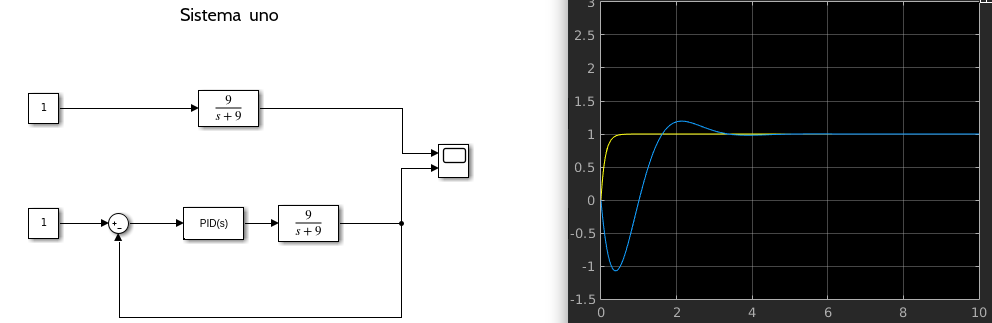
\includegraphics[width=15cm]{sim1.png}
\label{fig:tubes}
\end{floatrow}
\end{figure}\hfill \break 

\end{center}\hfill \break 


Ejercicio 2: 

\begin{center}

\begin{figure}[h!]
\begin{floatrow}
%\caption{Poderosisima udeg}
\centering
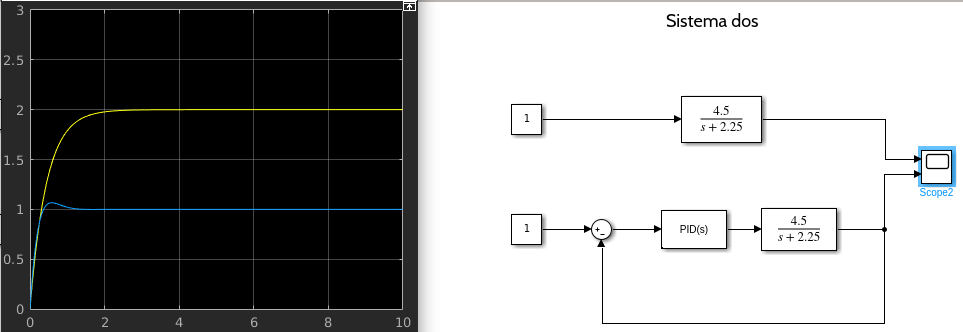
\includegraphics[width=13.1cm]{sim2.png}
\label{fig:tubes}
\end{floatrow}
\end{figure} 
\end{center}


Ejercicio 3: 

\begin{center}

\begin{figure}[h!]
\begin{floatrow}
%\caption{Poderosisima udeg}
\centering
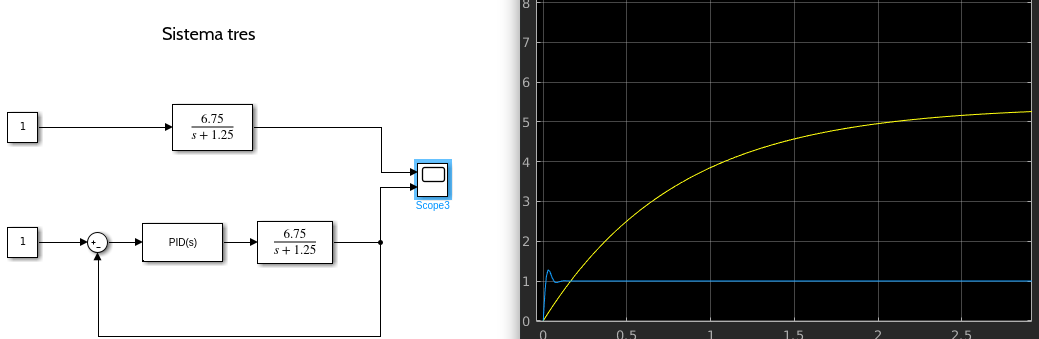
\includegraphics[width=13.1cm]{sim3.png}
\label{fig:tubes}
\end{floatrow}
\end{figure} 
\end{center}

Ejercicio 4: 

\begin{center}

\begin{figure}[h!]
\begin{floatrow}
%\caption{Poderosisima udeg}
\centering
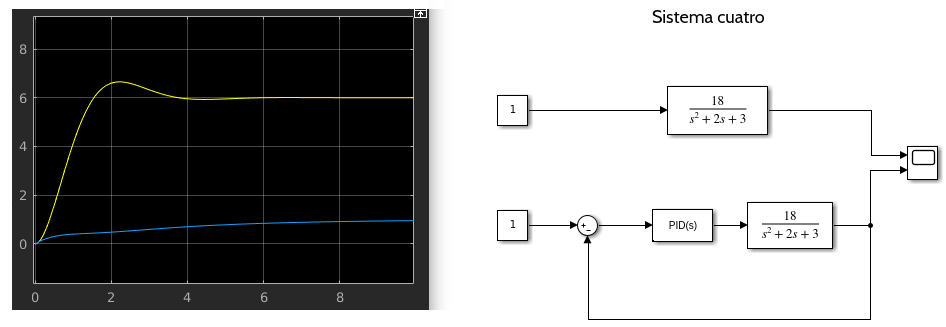
\includegraphics[width=13.1cm]{sim4.png}
\label{fig:tubes}
\end{floatrow}
\end{figure} 

\end{center} \hfill \break 



%%%%%%%%%%%%%%%%%%%%%%%%%%%%%%%%%%%%%%%%%%%%%%%%%%%%%%%%%%%%%%%%%%%%%%%%%%%%%%%%%%%%%%%%%%%%%%%%%%%%%%%%%%%%%%%%%%%%%%%%%
\section{Conclusión}

Se comprobo el uso del modelo Matemático de segundo orden de una función de transferencia asi como los parametros que describen dicha ecuación. \\ 
La tecnica de diseño de controladores PID por asignación de polos es eficiente porque basicamente tu defines un modelo ideal de como quieres que se comporte tu sistema y lo igualas a tu modelo real para encontrar las ganancias que hacen que tu sistema se comporte de la manera que quieres. \\ Este proceso es asignar los mismos polos ideales a los reales -En este documento llamados generales- del sistema.  

\begin{center}
\begin{figure}[h!]
\begin{floatrow}
%\caption{Mark-1: "Robot de exploración espacial"}
\centering
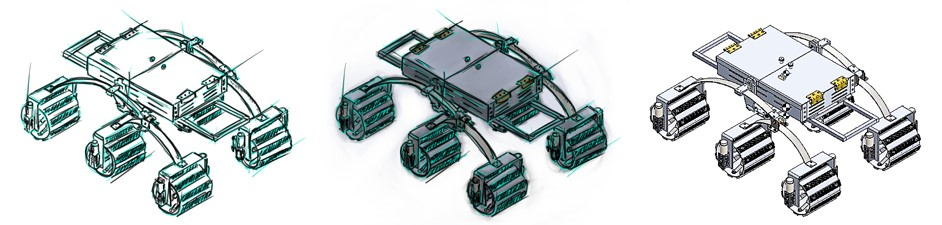
\includegraphics[width=13.1cm]{mark-1.jpeg}
\label{fig:tubes}
\end{floatrow}
\end{figure} 
\end{center} \hfill \break 
 
 
%%%%%%%%%%%%%%%%%%%%%%%%%%%%%%%%%%%%%%%%%%%%%%%%%%%%%%%%%%%%%%%%%%%%
\section{Referencias}
[1] N. Nise, Control systems engineering, 6th ed. Norman Nise, 2006. \\ 

[2] «Aplicaciones PID 4r4r». Rocatek. 5 de octubre de 2010. \\

[3] http://www.mathworks.es/discovery/pid-control.html \\ \ Control PID con MATLAB y Simulink \\


[4] https://es.wikipedia.org/wiki/Controlador\_PID \\ 


\end{document}
